
\chapter{Digital Step Attenuator 2}
\label{ch:dsa2}
\raggedbottom

This second DSA uses the same structure as the previous DSA~\cite{4639533_ch6,8354931_ch6}, with a binary architecture and a pi attenuator.

\begin{figure}[H]
    \centering
    \vspace{-4pt}
    
\includegraphics[width=0.75\textwidth]{binary_architecture.png}
    \caption{Binary architecture}
    \label{fig:dsa2_binary}
\end{figure}

\begin{figure}[H]
    \centering
    \vspace{-4pt}
    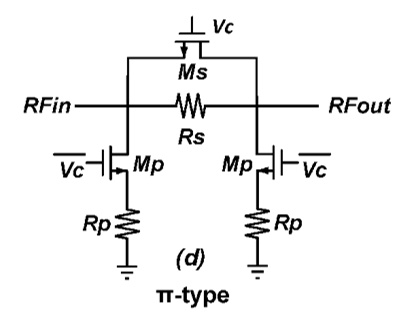
\includegraphics[width=0.75\textwidth]{chapter4/images/fig5.png}
    \caption{Pi attenuator}
    \label{fig:dsa2_pi}
\end{figure}

%=============================================================
\section{Proposed Full Layout}
\label{sec:dsa2_layout}

\begin{figure}[H]
    \centering
    \vspace{-4pt}
    
\includegraphics[width=0.75\textwidth]{dsa2_layout.png}
    \caption{Full DSA layout}
    \label{fig:dsa2_layout}
\end{figure}

%=============================================================
\section{Post-Layout Results}
\label{sec:dsa2_post_layout}

%-------------------------------------------------------------
\subsection{$S_{11}$ Across Frequency}
\label{subsec:dsa2_S11}

\begin{figure}[H]
    \centering
    \vspace{-4pt}
    
\includegraphics[width=0.75\textwidth]{S11_TT_DSA2.png}
    \caption{$S_{11}$ across frequency}
    \label{fig:dsa2_S11}
\end{figure}

%-------------------------------------------------------------
\subsection{$S_{22}$ Across Frequency}
\label{subsec:dsa2_S22}

\begin{figure}[H]
    \centering
    \vspace{-4pt}
    
\includegraphics[width=0.75\textwidth]{S22_TT_DSA2.png}
    \caption{$S_{22}$ across frequency}
    \label{fig:dsa2_S22}
\end{figure}

%-------------------------------------------------------------
\subsection{Attenuation States Across Frequency}
\label{subsec:dsa2_atten_states}

\begin{figure}[H]
    \centering
    \vspace{-4pt}
    
\includegraphics[width=0.75\textwidth]{S21_TT_DSA2.png}
    \caption{Attenuation states across frequency}
    \label{fig:dsa2_atten_states}
\end{figure}

%-------------------------------------------------------------
\subsection{DNL Across States for Different Frequencies}
\label{subsec:dsa2_DNL}

\begin{figure}[H]
    \centering
    \vspace{-4pt}
    
\includegraphics[width=0.75\textwidth]{DNL_TT_DSA2.png}
    \caption{DNL across states for different frequencies}
    \label{fig:dsa2_DNL}
\end{figure}

%-------------------------------------------------------------
\subsection{OIP3 Across Frequency for IL State}
\label{subsec:dsa2_OIP3}

\begin{figure}[H]
    \centering
    \vspace{-4pt}
    
\includegraphics[width=0.75\textwidth]{OIP3__DSA2.png}
    \caption{OIP3 across frequency for IL state}
    \label{fig:dsa2_OIP3}
\end{figure}

%-------------------------------------------------------------
\subsection{OP1dB Across Frequency for IL State}
\label{subsec:dsa2_OP1dB}

\begin{figure}[H]
    \centering
    \vspace{-4pt}
    
\includegraphics[width=0.75\textwidth]{OP1DB_dsa.png}
    \caption{OP1dB across frequency for IL state}
    \label{fig:dsa2_OP1dB}
\end{figure}

%-------------------------------------------------------------
\subsection{DNL Across SS/Hot Corner}
\label{subsec:dsa2_DNL_SS}

\begin{figure}[H]
    \centering
    \vspace{-4pt}
    
\includegraphics[width=0.75\textwidth]{dnl_sshot.png}
    \caption{DNL across SS/Hot corner}
    \label{fig:dsa2_DNL_SS}
\end{figure}

%-------------------------------------------------------------
\subsection{DNL Across FF/Cold Corner}
\label{subsec:dsa2_DNL_FF}

\begin{figure}[H]
    \centering
    \vspace{-4pt}
    
\includegraphics[width=0.75\textwidth]{dnl_ffcold__DSA2.png}
    \caption{DNL across FF/Cold corner}
    \label{fig:dsa2_DNL_FF}
\end{figure}
%\renewcommand{\bibname}{References}
%\bibliographystyle{ieeetr}
%\bibliography{chapter6/refs}
